%%%%%%%%%%%%%%%%%%%%%%%%%%%%%%%%%%%%%%%%%%%%%%%%%%%%%%%%%%%%%%%%%%%%%%%%%%%
%% This file is part of the book
%%
%% Algorithmic Graph Theory
%% http://code.google.com/p/graph-theory-algorithms-book/
%%
%% Copyright (C) 2009, 2010, 2011 Minh Van Nguyen <nguyenminh2@gmail.com>
%%
%% See the file COPYING for copying conditions.
%%%%%%%%%%%%%%%%%%%%%%%%%%%%%%%%%%%%%%%%%%%%%%%%%%%%%%%%%%%%%%%%%%%%%%%%%%%

\documentclass{article}

\usepackage{tikz}
\usetikzlibrary{external}
\tikzexternalize{vertex-disjoint-union-K15-W4}

\begin{document}

\begin{figure}
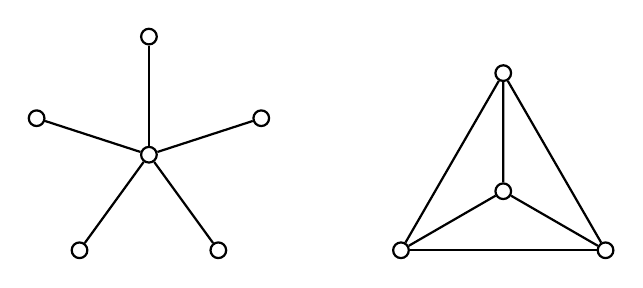
\begin{tikzpicture}
[nodeDecorate/.style={shape=circle,inner sep=2pt,draw,thick},%
  lineDecorate/.style={-,thick},%
  scale=1.5]
%%
%% complete bipartite graph K_{1,5}
%% nodes or vertices
\foreach \nodename/\x/\y in {
  1/0.9510/0.3090, 2/0/1, 3/-0.9510/0.3090, 4/-0.5877/-0.8090,
  5/0.5877/-0.8090, 6/0/0}
{
  \node (\nodename) at (\x,\y) [nodeDecorate] {};
}
%% edges or lines
\path
\foreach \startnode/\endnode in {1/6, 2/6, 3/6, 4/6, 5/6}
{
  (\startnode) edge[lineDecorate] node {} (\endnode)
};
%%
%% wheel graph W_4
%% nodes or vertices
\foreach \nodename/\x/\y in {
  1/3.866/-0.809, 2/3/0.691, 3/2.134/-0.809, 4/3/-0.309}
{
  \node (\nodename) at (\x,\y) [nodeDecorate] {};
}
%% edges or lines
\path
\foreach \startnode/\endnode in {1/2, 1/3, 1/4, 2/3, 2/4, 3/4}
{
  (\startnode) edge[lineDecorate] node {} (\endnode)
};
\end{tikzpicture}
\end{figure}

\end{document}
